\documentclass[12pt,a4paper]{book}
\usepackage[utf8]{inputenc}
\usepackage{geometry}
\usepackage{enumitem}
\usepackage[dvipsnames]{xcolor}
\usepackage[T1]{fontenc}
\usepackage{textcomp}
\usepackage{tgtermes}
\usepackage{graphicx, wrapfig}
\graphicspath{{images/}}
\usepackage{float} %provide us with the option H
\usepackage{lipsum} %for dummy text
\usepackage{tcolorbox}
\usepackage{siunitx}
\newtcolorbox{titlecolorbox}[1]{ %the box around chapter
	coltext=white,
	colframe=black,
	colback=black,
	boxrule=0pt,
	arc=0pt,
	notitle,
	width=4.8em,
	height=2.4ex,
	before=\hfill
}
\usepackage{pdfpages}
\usepackage{chngcntr}
\counterwithin{figure}{chapter}
\usepackage{fancyhdr}
\renewcommand{\chaptername}{Capítulo}
\usepackage{xcolor}

\usepackage[explicit]{titlesec}
\titleformat{\chapter}[display]
{\sffamily\Huge}
{}
{0pt}
{\begin{titlecolorbox}{}
		{\large\sffamily\MakeUppercase{\chaptername}}
	\end{titlecolorbox}
	\vspace*{-4.5ex}\noindent\rule{\textwidth}{0.4pt}
	\parbox[b]{\dimexpr\textwidth-4.8em\relax}{\raggedright\MakeUppercase{#1}}{\hfill\fontsize{60}{80}\selectfont\thechapter}
}
[]

\titleformat{name=\chapter,numberless}[display]
{\sffamily\Huge}
{}
{0pt}
{\begin{titlecolorbox}{}
		{\large\sffamily\MakeUppercase{\chaptername}}
	\end{titlecolorbox}
	\vspace*{-4.19ex}\noindent\rule{\textwidth}{0.4pt}
	\parbox[b]{\dimexpr\textwidth-4.8em\relax}{\raggedright\MakeUppercase{#1}}
}
[]

\titleformat{\section}[display]
{\sffamily\large}
{}
{0pt}
{\hrule\vspace*{0.25ex}\parbox[b]{\dimexpr\textwidth\relax}{\textcolor{darkgray}{\thesection}\quad\raggedright\bfseries\MakeUppercase{#1}}}
[\hrule]

\begin{document}
	
	\setcounter{chapter}{0}
	
	\chapter{Introducción a ARM Cortex-M}
	El grupo de núcleos de procesadores Arm\textregistered  Cortex\textregistered-M es una serie de núcleos optimizados para la eficiencia de energía y operaciones determinísticas. Es ampliamente usado en microcontroladores (MCUs) y también puede ser encontrado embebidos dentro de microprocesadores multi núcleo (MPUs).\\
	
	\noindent\begin{minipage}{0.7\textwidth}% adapt widths of minipages to your needs
		\noindent Desde los microcontroladores iniciales con núcleo Cortex\textregistered -M3 y la introducción de variantes de núcleos optimizados para \textbf{baja potencia}: como el Cortex\textregistered -M0 y el Cortex\textregistered -M0+, núcleos optimizados para un mayor \textbf{rendimiento}: como el Cortex\textregistered -M7, núcleos para aplicaciones en \textbf{tiempo real} como el Cortex\textregistered -M4 o enfocados en \textbf{seguridad} como el Cortex\textregistered -M33. La arquitectura Arm\textregistered Cortex\textregistered -M es la arquitectura estándar de facto para MCUs de 32 bits de propósito general.
	\end{minipage}%
	\begin{minipage}{0.3\textwidth}% adapt widths of minipages to your needs
		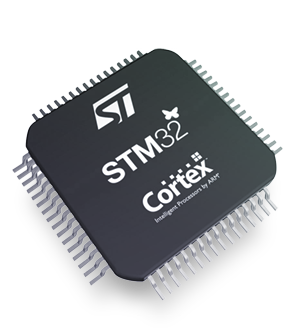
\includegraphics[width=\linewidth]{image5}
	\end{minipage}%
	
	\noindent Las principales ventajas de tener la arquitectura estandarizada Arm\textregistered Cortex\textregistered -M son:
	
	\begin{itemize}[noitemsep]
		\item Los ingenieros pueden transferir fácilmente su código de una serie de MCU a otra. Pueden elegir la correcta compensación entre eficiencia energética, rendimiento computacional, seguridad y un amplio rango de periféricos para sus sistemas.
		\item Aprovechar un rico ecosistema de proveedores de microcontroladores y de proveedores de herramientas de software y hardware.
		\item Acelerar la innovación en aplicaciones embebidas.
	\end{itemize}


	\noindent STMicroelectronics fue uno de los primeros en adoptar los núcleos Arm\textregistered Cortex\textregistered -M y actualmente lidera el mercado con la mayor cartera de MCUs Cortex\textregistered -M de 32 bits.
	
	\section{Arm Cortex\textregistered-M3}
	El núcleo de procesador de 32 bits Arm\textregistered Cortex\textregistered-M3 está diseñado para aplicaciones de costo limitado de \textbf{alto rendimiento} y \textbf{procesamiento en tiempo real} y capaz de manejar tareas complejas. Cualquier microcontrolador Arm \textregistered Cortex\textregistered-M3 ofrece una alta escalabilidad combinada con combinado con un balance óptimo entre rendimiento y costo.
	 

	\chapter{Fundamentos del STM32}
	
	\section{Timers e Interrupciones}
	Los timers son una de las características más importantes en los microcontaroladores modernos. Nos permiten medir cuánto tiempo toma en ejecutarse cierta tarea, controlar con precisión la sincronización de un pin e incluso correr sistemas operativos.\\
	
	 \noindent La línea de microcontroladores STM32 de STMicroelectronics no son la excepción: cada controlador ofrece un conjunto completo de timers para su uso.
	 
	 \subsection{Timers basics}
	 Un timer (a veces referido como contador) es una pieza especial de hardware dentro de la mayoría de microcontroladores. Su función es simple: estos cuentan (en forma ascendente o descendente, dependiendo de su configuración). Por ejemplo, un timer de 8 bits contará desde 0 hasta 255. La mayoría de los timers se "reiniciarán" una vez que alcanzan su valor máximo, así, nuestro contador de 8 bits iniciaría de nuevo desde 0 una vez que alcance el valor de 255. \\
	 
	 \noindent Es posible aplicar una variedad de configuraciones a la mayoría de los timers para cambiar la forma en que estos funcionan. Estas configuraciones usualmente se aplican en registros de funciones especiales dentro del microcontrolador. Por ejemplo, en lugar de contar hasta un máximo de 255, le puedes indicar al timer que quieres reiniciar la cuenta una vez que llegue a 100. Adicionalmente, puedes conectar más hardware o periféricos dentro del microcontrolador al timer como el alternar automáticamente el estado de un pin cuando el timer llegue a la cuenta indicada.
	 
	 \noindent Alguna de las funciones que se pueden lograr con un timer son:
	 \begin{itemize}[noitemsep]
	 	\item Output Compare (OC): alternar el estado de un pin cuando el timer alcanza un cierto valor
	 	\item Input Campute (IC): medir el número de conteos de un timer entre eventos sobre un pin
	 	\item Pulse Width Modulation (PWM): alternar el estado de un pin cuando el timer alcanza un cierto valor y al reiniciar. Ajustando el tiempo de encendido vs el tiempo de apagado (duty cycle) se puede controlar efectivamente la cantidad de energía que pasará a través de otro dispositivo. 
	 \end{itemize}
	 
	 \subsubsection{Prescaler}
	 ¿Qué tan rápido se ejecutan los timers? Depende de qué tan rápido le indique uno. Todos los timers requieren de algún tipo de reloj. La mayoría estarán conectados al reloj principal de la CPU del microcontrolador (otros, colo los relojes en tiempo real (real time clock) tienen sus propieas fuentes de reloj). Un timer marcará (incrementará en uno) cada vez que reciba un pulso del reloj. \\
	 
	 \noindent Supongamos que tenemos un reloj principal (HCLK) de  $\SI{80}{MHz}$, y podríamos tener un timer ejecutándose a  $\SI{80}{MHz}$, pero esto puede ser demasiado rápido para nuestras aplicaciones. Un timer de 16 bits puede contar hasta $2^{16}=65,535$ antes de que se reinicie, esto significa que podemos medir eventos no más grandes que $\frac{1}{ \SI{80}{MHz}}\times 65535 = \SI{819}{\mu\s}$.
	 
	 \noindent Si deseamos medir tiempos más largos, necesitamos usar un prescaler, el cual es una pieza de hardware que divide los pulsos de la fuente de reloj. Por ejemplo, un prescaler de 80 convertiría un reloj de $\SI{80}{MHz}$ en un reloj de $\SI{1}{MHz}$
	 
	 \begin{figure}[H]
	 	\centering
	 	
\includegraphics[scale=0.8]{image1}
	 	\caption{Uso del prescaler para disminuir los pulsos del reloj}
	 	\label{fig:pic1.1}
	 \end{figure}
	 
	 \noindent Ahora nuestro timer daría un pulso cada $\frac{1}{\SI{1}{MHz}} =\SI{1}{\mu\s} $ y asumiendo un timer de 16 bits entonces sería capaz de cronometrar eventos de hasta un máximo de $\frac{1}{ \SI{1}{MHz}}\times 65535 = \SI{65.5}{\ms}$.
	 
	 \subsubsection{Escogiendo un timer}
	 Si observas el datasheet de tu microcontrolador, encontrarás una sección hablando acerca de los timers disponibles que éste posee. Por ejemplo, en la hoja de datos del microcontrolador STM32F303RE, la sección 3.18 nos proporciona información de los timers a nuestra disposición.
	 
	 \begin{figure}[H]
	 	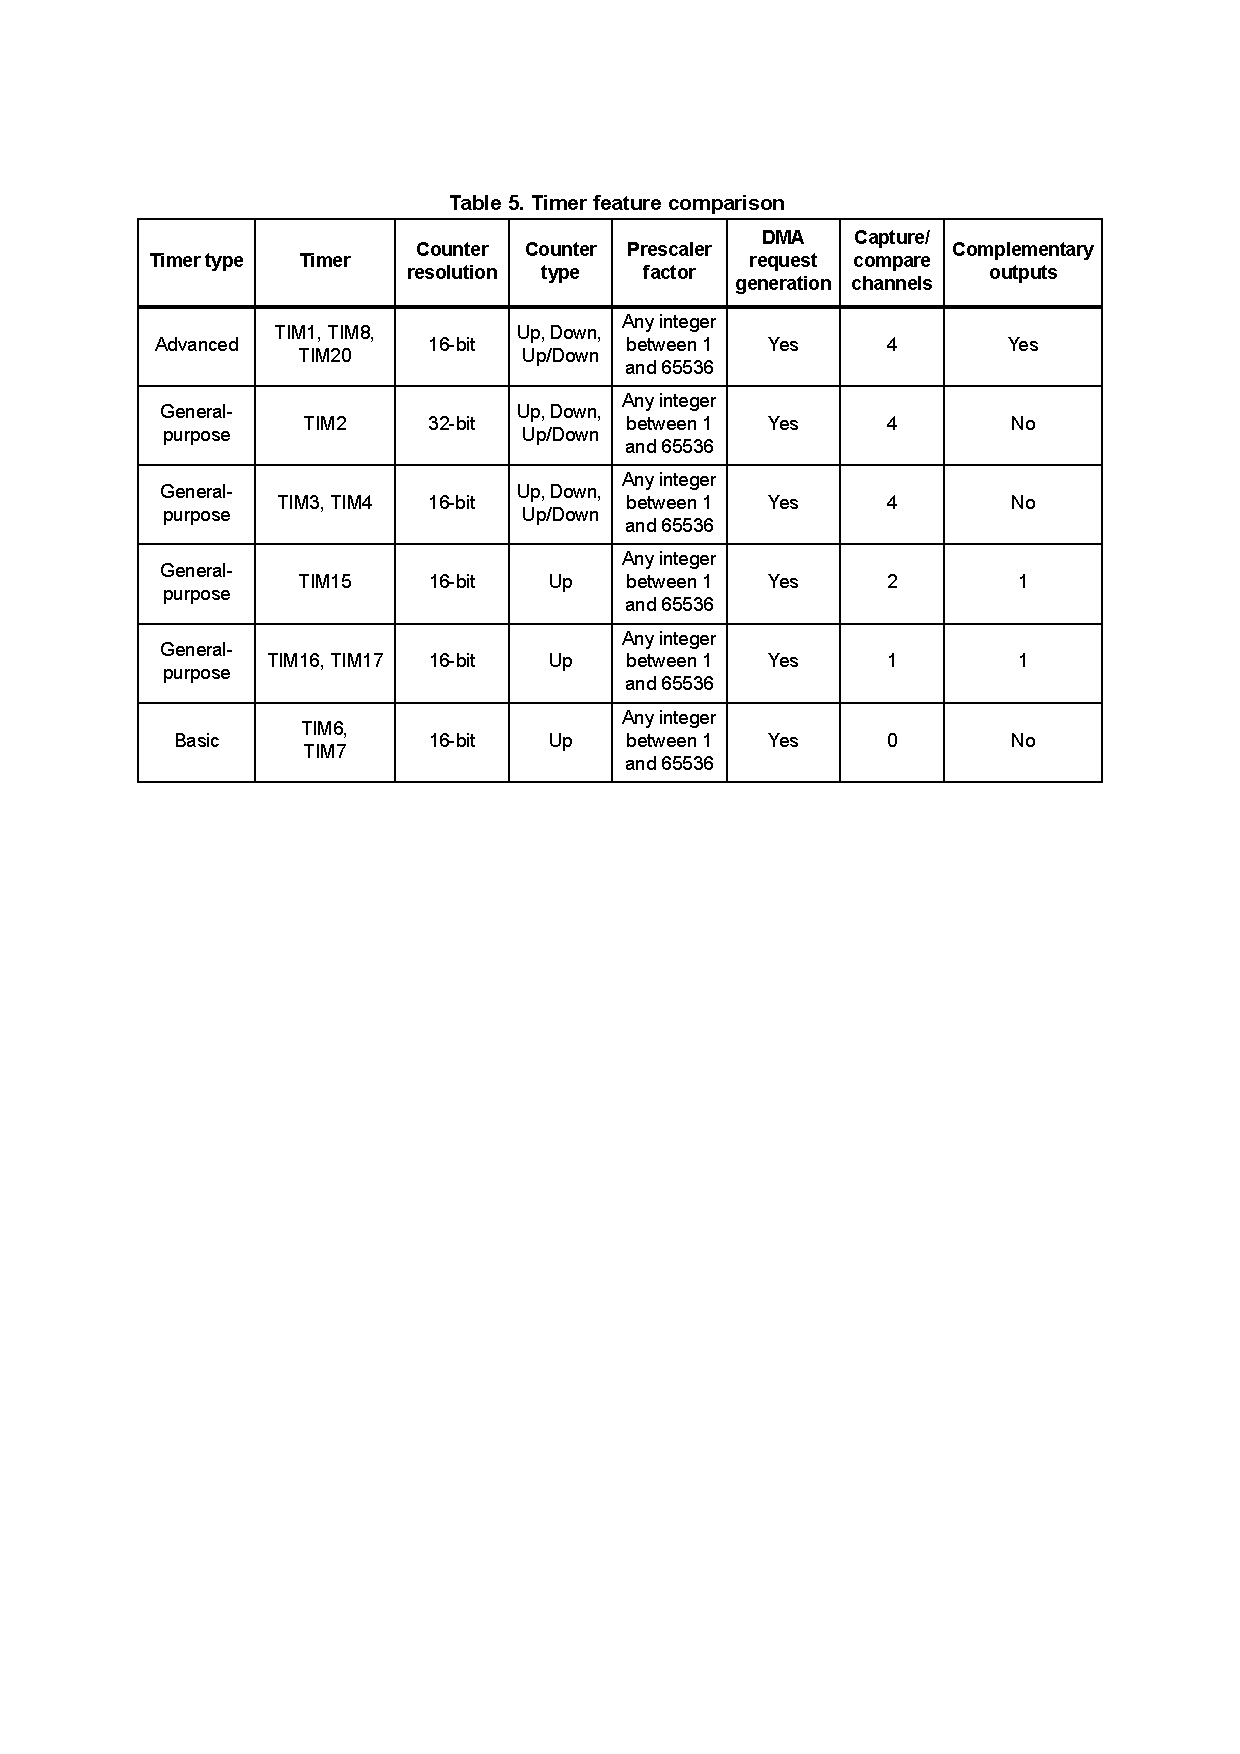
\includegraphics[scale = 0.89]{image3.pdf}
	 \end{figure}
	 
	 \subsection{LEDs blinking usando timers}
	 En este ejercicio de práctica se utilizán los timers \texttt{TIM2}, \texttt{TIM3} y \texttt{TIM4} para hacer parpadear tres LEDs a diferentes frecuencias. Dichas frecuencias serán establecidas en  $\SI {0.5}{s}$ ( $\SI {2}{Hz}$), $\SI {1}{s}$ ($\SI {1}{Hz}$) y  $\SI {2}{s}$ ($\SI {0.5}{Hz}$) respectivamente. 
	 
	 \subsubsection{Nuevo proyecto}
	 Una vez abierto nuestro IDE, en la pestaña de \textbf{Board selector} buscamos la tarjeta de desarrollo \texttt{NUCLEO-F303RE} creamos un nuevo proyecto con el nombre de \texttt{LEDs\_Binking} \texttt{\_With\_Timers}
	 \begin{figure}[H]
	 	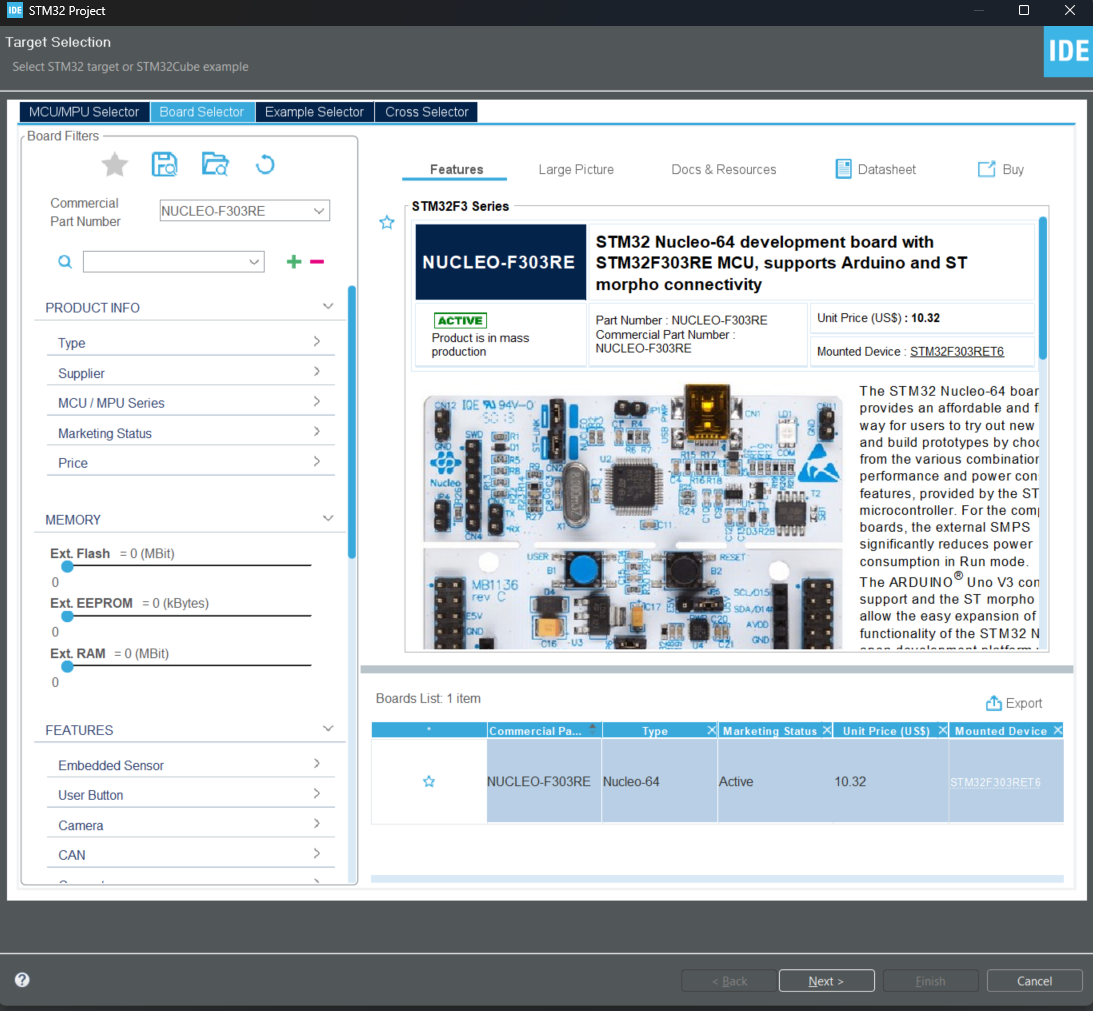
\includegraphics[width=\linewidth]{image6}
	 \end{figure}
	 
	 \noindent En la ventana de \textbf{Device Configuration Tool} podremos encontrar una figura del microcontrolador utilizado con todos los pines disponibles para ser configurados a nuestro criterio. Dentro de la sección de \texttt{Timers} seleccionamos el \texttt{Timer2}. los parámetros a configurar dentro de la subsección de \textbf{Mode} son:
	 
	 \begin{itemize}[noitemsep]
	 	\item \textbf{Clock source:} Establecerla como \textit{Internal Clock}
	 	\item \textbf{Channel1:} Establecerlo como \textit{PWM Generation CH1}
	 \end{itemize}
	 
	 \noindent Nuestra meta es generar una señal de reloj con una frecuencia de $\SI {0.5}{Hz}$. Nuestro reloj principal tiene una frecuencia de $\SI {72}{MHz}$, sin embargo, esta es una frecuencia demasiado grande para nuestros propósitos.\\ 
	 
	 \noindent Para bajar dicha frecuencia de nuestro reloj principal a tan sólo $\SI {0.5}{Hz}$ haremos uso del \textbf{prescaler} y del \textbf{Autoreload register}, parámetros que se encuentran en la subsección de \textbf{Configuration}.
	 
	  \begin{figure}[H]
	 	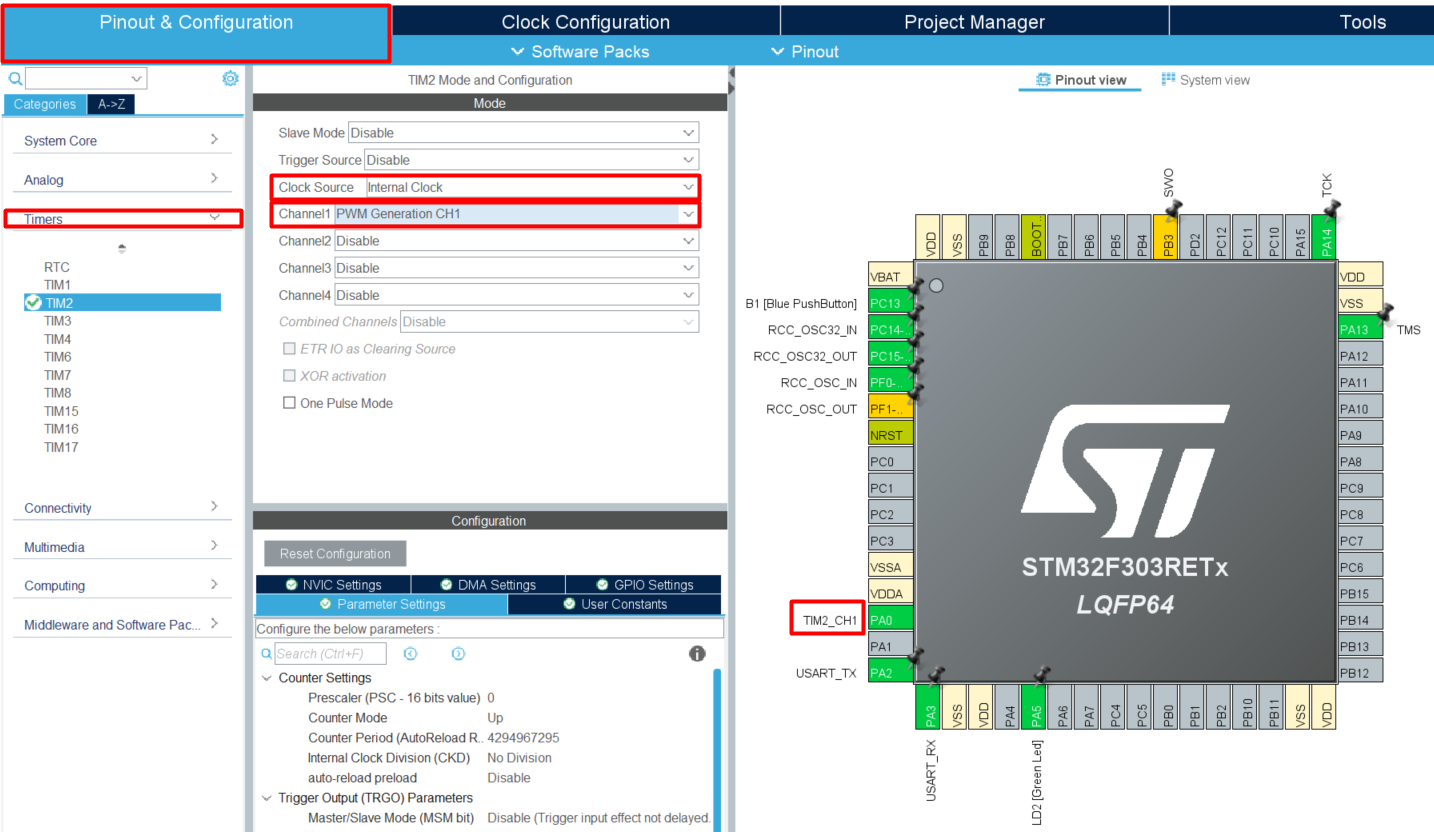
\includegraphics[width=\linewidth]{image7}
	 \end{figure}
	 
	 
\end{document}